
\documentclass[letterpaper, 10 pt, conference]{ieeeconf}  % Comment this line out
\usepackage{graphicx}
                                                          % if you need a4paper

\overrideIEEEmargins
% See the \addtolength command later in the file to balance the column lengths
% on the last page of the document

\usepackage[utf8]{inputenc}
\usepackage[T1]{fontenc}

% The following packages can be found on http:\\www.ctan.org
\usepackage{graphics} % for pdf, bitmapped graphics files
%\usepackage{epsfig} % for postscript graphics files
%\usepackage{mathptmx} % assumes new font selection scheme installed
%\usepackage{mathptmx} % assumes new font selection scheme installed
\usepackage{amsmath} % assumes amsmath package installed
\usepackage{amssymb}  % assumes amsmath package installed

\title{\LARGE \bf
Clasificación de MRI con Redes Neuronales Convolucionales para Tipos de Cáncer
}

\author{Jhon Edwuard Zacipa Casas José Luis Sarta Alvarez  y Marco Julio Gómez Amado }

\usepackage{float}
\begin{document}

\maketitle
\thispagestyle{empty}
\pagestyle{empty}



%%%%%%%%%%%%%%%%%%%%%%%%%%%%%%%%%%%%%%%%%%%%%%%%%%%%%%%%%%%%%%%%%%%%%%%%%%%%%%%%
\section{Introducción}

En los últimos años, el campo de la visión por computadora y el aprendizaje profundo ha experimentado un crecimiento exponencial, revolucionando aplicaciones críticas en la biomedicina y la bioinformática. A pesar de los significativos avances en el análisis automatizado de imágenes médicas, persisten desafíos importantes, tales como la alta carga computacional en el manejo de datos volumétricos por Imágenes de Resonancia Magnética (MRI), la escasez de volúmenes masivos de datos etiquetados y la necesidad de estandarizar procesos para mitigar el sobreajuste en modelos predictivos.

Dentro de este panorama, el problema específico abordado en este informe es la clasificación automatizada de neoplasias cerebrales a partir de imágenes de resonancia magnética (MRI), categorizadas en cuatro clases principales (Glioma, Healthy, Meningioma y Pituitary). La relevancia de este desafío radica en la necesidad de contar con herramientas diagnósticas rápidas y de alta precisión que reduzcan la variabilidad subjetiva. 

El presente estudio presenta el diseño, entrenamiento y evaluación comparativa de tres arquitecturas de aprendizaje profundo: una CNN personalizada desde cero, un modelo ResNet18 con extracción de características, y una estrategia propuesta de ResNet18 con Fine-Tuning parcial en el bloque layer4. Los principales aportes de este trabajo consisten en el logro de una precisión global del $98.0\%$ con convergencia óptima en tan solo 5 épocas, respaldada por un análisis riguroso de métricas cuantitativas y validada mediante técnicas de explicabilidad visual con Grad-CAM para garantizar la confiabilidad clínica del modelo.


\section{Metodología}

2.1 Enfoque General del Estudio. 
El presente estudio propone un enfoque comparativo basado en Transfer Learning y Fine-Tuning para la clasificación automatizada de tumores cerebrales a partir de imágenes médicas. El flujo experimental evalúa y contrasta tres variantes: una CNN personalizada, un modelo de extracción de características estáticas y una estrategia propuesta de ajuste fino parcial (Fine-Tuning en el bloque layer4), la cual optimiza la representación espacial de la lesión sin alterar las características generales de bajo nivel.

2.2 Datos, Preprocesamiento y División.
Se utilizó un conjunto de datos de acceso público compuesto por $7,023$ imágenes de resonancia magnética (MRI)\footnote{\url{https://www.kaggle.com/datasets/rm1000/brain-tumor-mri-scans}}, distribuidas en cuatro clases clínicas: \textit{Glioma}, \textit{Healthy}, \textit{Meningioma} y \textit{Pituitary}.

\textbf{Preprocesamiento:} Las imágenes fueron sometidas a un pipeline de transformación inicial consistente en un redimensionamiento uniforme a una resolución de \texttt{img\_size} mediante la función \texttt{transforms.Resize} y su conversión a tensores normalizados en el rango de $[0.0, 1.0]$ mediante \texttt{transforms.ToTensor()}.

\textbf{División del Conjunto:} Los datos fueron segmentados en conjuntos independientes para garantizar una evaluación imparcial durante las fases de entrenamiento, validación y prueba (con un conjunto de evaluación final compuesto por $1,405$ imágenes).

2.3 Arquitectura de los Modelos Evaluados.
Se implementaron y compararon tres arquitecturas de aprendizaje profundo en PyTorch:
Modelo 1 (CNN Personalizada): Una red neuronal convolucional diseñada desde cero compuesta por tres capas convolucionales secuenciales, activaciones ReLU y bloques de agrupamiento (max-pooling).
Modelo 2 (ResNet18 - Feature Extraction): Utiliza la arquitectura base ResNet18 con el tronco convolucional completamente congelado, manteniendo fijos los pesos pre-entrenados y entrenando únicamente un clasificador lineal adaptado al problema.
Modelo 3 (ResNet18 - Fine-Tuning Parcial / modelo propuesto): Modifica la arquitectura ResNet18 congelando las capas iniciales de bajo nivel (layer1 a layer3) y descongelando selectivamente el bloque convolucional superior (layer4) junto con un clasificador rediseñado. Este clasificador consta de una capa lineal de $512 \to 128$ neuronas, función de activación ReLU, una tasa de abandono (Dropout) del $0.3$ para mitigar el sobreajuste, y una capa lineal de salida de $128 \to 4$ clases correspondientes a las patologías evaluadas.

2.4 Estrategia de Entrenamiento y Evaluación.
Hiperparámetros y Optimizador: El entrenamiento del Modelo 3 se configuró utilizando el optimizador Adam con una tasa de aprendizaje ($\text{lr}$) de $1\times 10^{-4}$ y una función de pérdida de entropía cruzada (Cross-Entropy Loss). El proceso se ejecutó de forma eficiente a lo largo de un ciclo corto de $5$ épocas debido a la rápida convergencia.
Procedimiento de Validación: Se empleó un conjunto de validación independiente monitoreado por época para registrar las curvas de aprendizaje (accuracy y loss).
Métricas de Evaluación: Para cuantificar el desempeño de los clasificadores, se utilizaron la Precisión Global (Accuracy), y las métricas por clase de F1-Score, además de promedios macro y ponderados para evaluar la sensibilidad ante las clases.

2.5 Análisis Adicionales y Explicabilidad (Grad-CAM)
Como parte de los estudios analíticos adicionales para evaluar la contribución de los componentes del modelo y su fiabilidad diagnóstica, se incorporó la técnica de explicabilidad Grad-CAM (Gradient-weighted Class Activation Mapping). Esta herramienta evalúa los gradientes que fluyen hacia el último bloque convolucional (layer4), generando mapas de calor superpuestos sobre las MRI con el fin de verificar empíricamente que el modelo focaliza su atención en las regiones tumorales reales y no en el contorno o en ruido de fondo.

\section{Resultados}

Los experimentos evaluaron el desempeño de las tres arquitecturas sobre el conjunto de prueba independiente ($1,405$ imágenes).

3.1 Tabla Comparativa de Modelos. 
La Tabla I resume el rendimiento cuantitativo global y por clases de los tres enfoques experimentales evaluados.
\begin{table}[htbp]
    \centering
    \caption{Comparativa de rendimiento y especificaciones de los modelos evaluados.}
    \label{tab:comparativa_modelos}
    \resizebox{\columnwidth}{!}{%
    \begin{tabular}{|l|c|c|c|}
        \hline
        \textbf{Métrica / Enfoque} & \textbf{Modelo 1: CNN} & \textbf{Modelo 2: Feat. Ext.} & \textbf{Modelo 3: Fine-Tuning} \\ \hline
        Estrategia & Desde cero & Tronco congelado & Bloque \texttt{layer4} \\ \hline
        Épocas & 8 & 8 & \textbf{5} \\ \hline
        Precisión Global & 96.0\% & 91.0\% & \textbf{98.0\%} \\ \hline
        F1-Score (Glioma) & 0.93 & 0.88 & \textbf{0.96} \\ \hline
        F1-Score (Healthy) & 0.98 & 0.98 & \textbf{0.99} \\ \hline
        F1-Score (Meningioma) & 0.90 & 0.83 & \textbf{0.95} \\ \hline
        F1-Score (Pituitary) & 0.97 & 0.93 & \textbf{0.99} \\ \hline
    \end{tabular}%
    }
\end{table}
Los resultados demuestran que, si bien una arquitectura entrenada desde cero ofrece un desempeño competitivo ($96.0\%$), la extracción pura de características limita el aprendizaje ($91.0\%$). En contraste, el Modelo 3 (Fine-Tuning) maximiza la precisión global ($98.0\%$) y eleva significativamente el F1-score en clases complejas como el Meningioma ($0.95$)

3.2 Curvas de Aprendizaje.
El Modelo 3 (Fine-Tuning parcial) alcanzó una precisión global del $98.0\%$. El análisis del proceso de optimización se refleja en las curvas de aprendizaje
\begin{figure}[htbp]
    \centering
    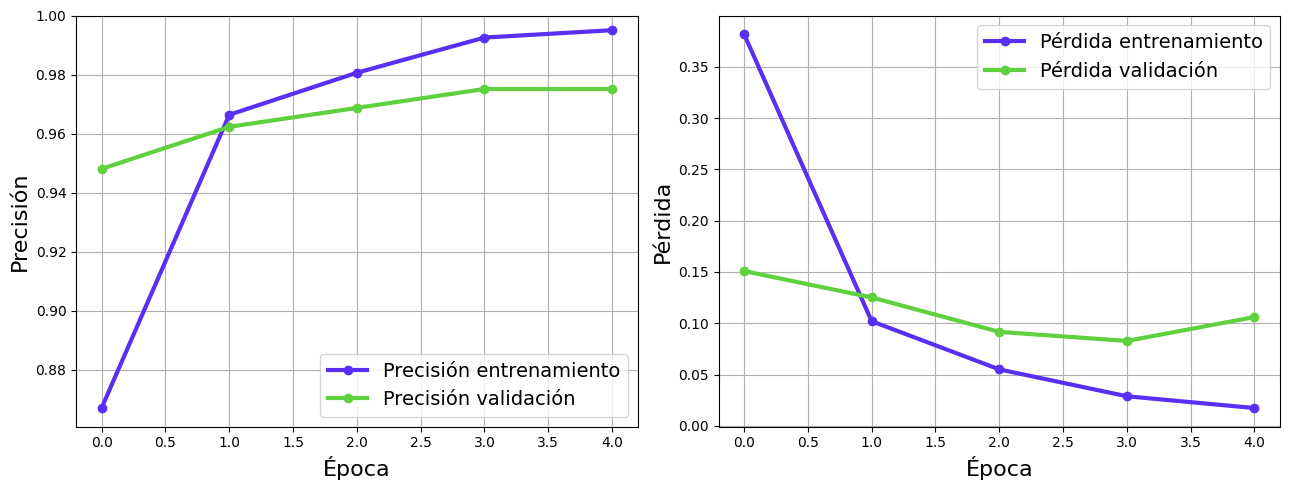
\includegraphics[width=0.50\textwidth]{curvas_aprendizaje.png}
    \caption{Evolución de la precisión y función de pérdida en entrenamiento y validación del Modelo 3.}
    \label{fig:curvas}
\end{figure}
Las curvas evidencian una convergencia eficiente en la época 4, registrando una pérdida de validación de $0.083$ y estabilizando la precisión de validación entre el $97.5\%$ y el $98.0\%$, lo que confirma la ausencia de sobreajuste severo.

3.3 Análisis Cualitativo y Explicabilidad (Grad-CAM). 
Para validar la interpretabilidad clínica del modelo, se empleó Grad-CAM sobre las imágenes de prueba:
\begin{figure}[htbp]
    \centering
    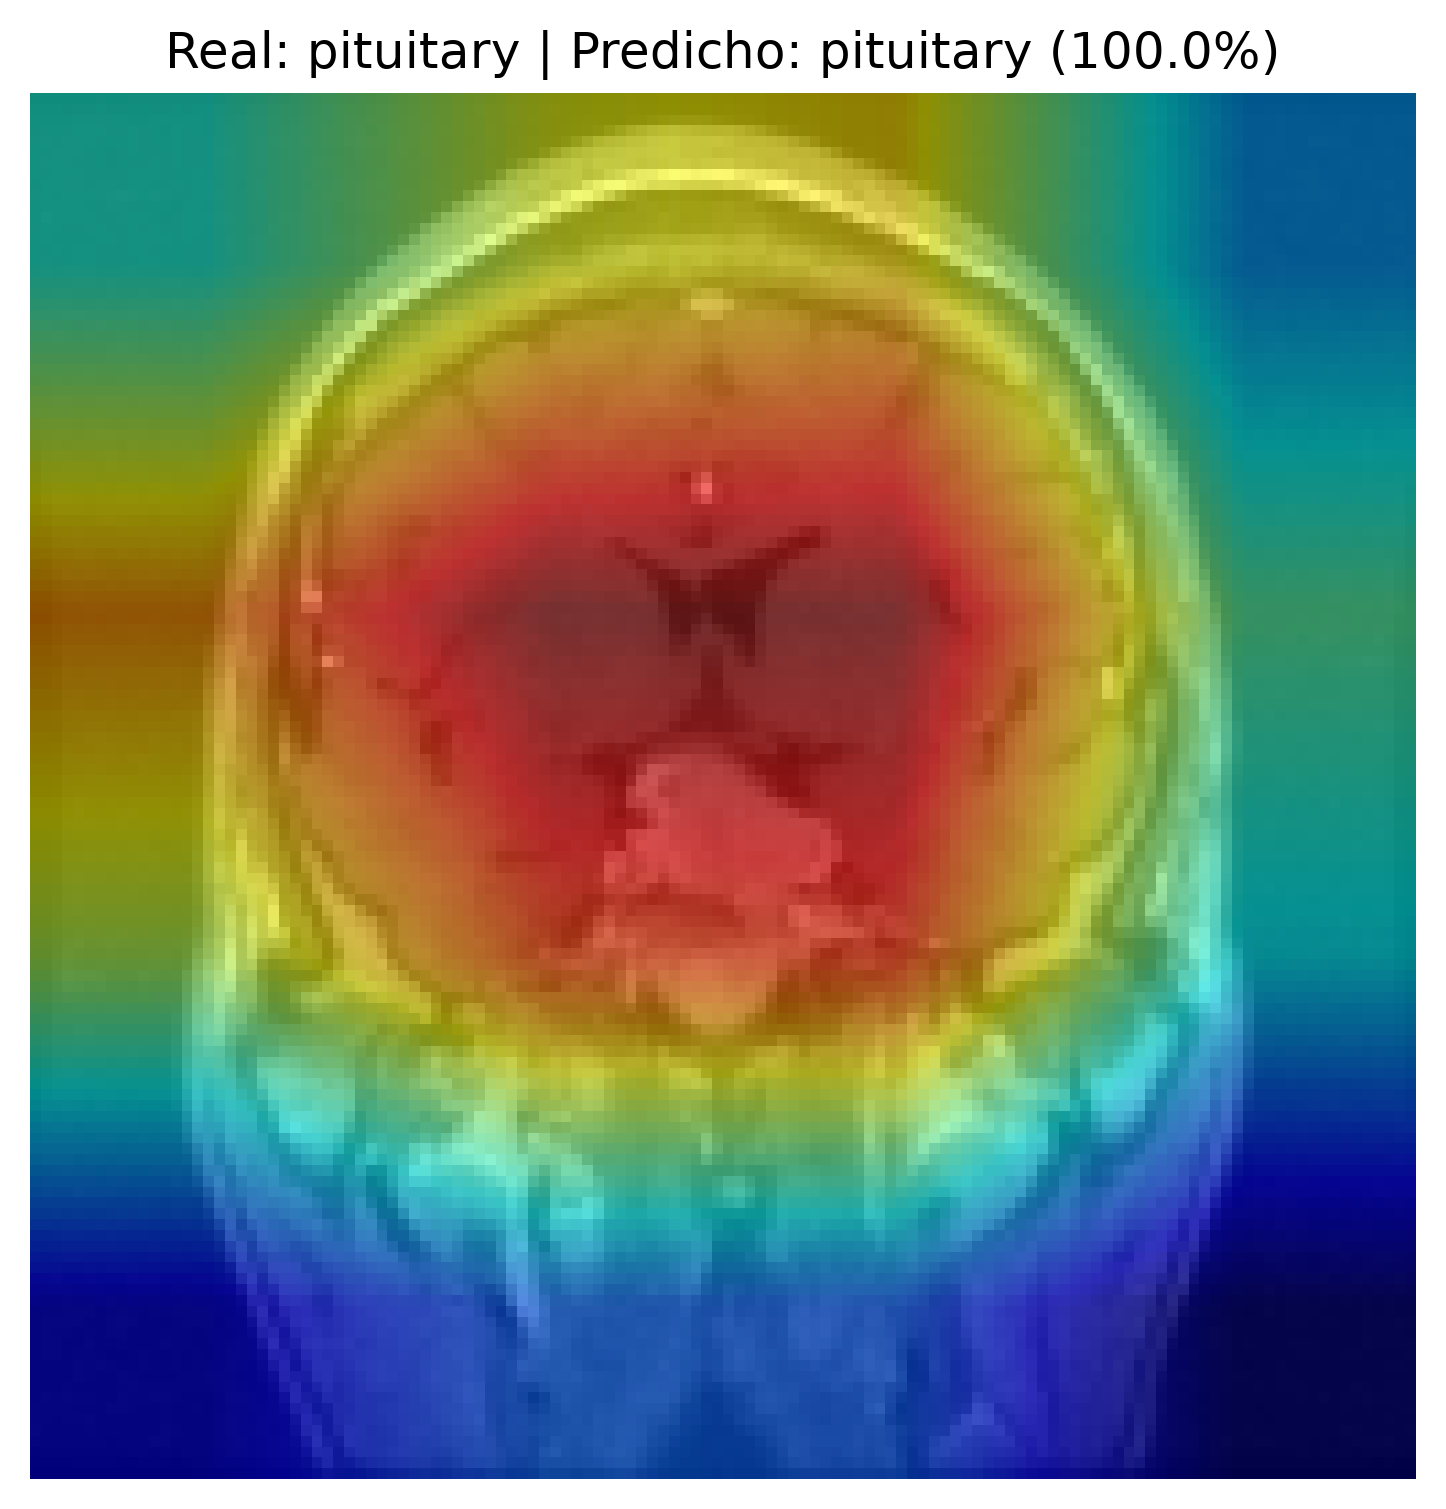
\includegraphics[width=0.30\textwidth]{gradcam_verificacion.png}
    \caption{Mapa de activación Grad-CAM (Clase Real: 3 | Predicho: 3 con 99.9\% de confianza).}
    \label{fig:gradcam}
\end{figure}
La evaluación visual demostró que el modelo emite predicciones correctas respaldadas por una confianza del $99.9\%$ en la instancia evaluada (Clase 3). El mapa de calor confirma que el sistema concentra sus activaciones máximas estrictamente sobre la masa tumoral.
\section{Discusión}

4.1 Interpretación y Contextualización de los Hallazgos.
Los resultados obtenidos demuestran que la estrategia de Fine-Tuning parcial en el bloque layer4 de ResNet18 (Modelo 3) supera tanto al entrenamiento desde cero (Modelo 1) como a la extracción de características estáticas (Modelo 2), alcanzando una precisión global del $98.0\%$. 

Asimismo, la validación mediante Grad-CAM permitió demostrar que el sistema emite diagnósticos con una confianza del $99.9\%$ y concentra sus activaciones estrictamente sobre la masa tumoral.

4.2 Limitaciones del Estudio. 
A pesar del sólido desempeño alcanzado, es fundamental reconocer las siguientes limitaciones:
Representatividad de los Datos: Aunque el conjunto de datos utilizado comprende $7,023$ imágenes de resonancia magnética de acceso público, las fuentes pueden no reflejar completamente la variabilidad de equipos de resonancia, intensidades de campo magnético o artefactos de movimiento presentes en la práctica clínica real.

Sensibilidad a Hiperparámetros: El rendimiento estuvo acotado a una tasa de aprendizaje de $1\times 10^{-4}$ y al ajuste específico del bloque layer4; explorar esquemas de descongelación gradual (gradual unfreezing) podría refinar aún más el equilibrio entre estabilidad y adaptación.

Como líneas de trabajo futuro se propone: Incorporar técnicas avanzadas de aumento de datos (data augmentation), con el fin de enriquecer la variabilidad interpaciente, equilibrar clases minoritarias y mitigar sesgos.

Emplear conjuntos de datos provenientes de diferentes centros hospitalarios y equipos de resonancia magnética con distintas intensidades de campo magnético.

% Para la parte de referencias puedes usar un archivo .bib o seguir el formato que convenga

\begin{thebibliography}{99}

\bibitem{c1} Jon Krohn, Grant Beyleveld, Aglaé Bassens, 2019, ``Deep Learning Illustrated (capítulo 10),'' .
\bibitem{c2} W.-K. Chen, Linear Networks and Systems (Book style).	Belmont, CA: Wadsworth, 1993, pp. 123--135.

\end{thebibliography}




\end{document}
